\subsection{Giới thiệu về vector}
Xét một tình huống mà ở đó bạn di chuyển 3m về phía Bắc, sau đó đi tiếp 4m về phía Đông. Nếu như bạn chỉ quan tâm đến quãng đường mình đã đi được, ta chỉ đơn giản là lấy \(3+4=7\si{m}\). Tuy nhiên, khi ta xét đến \textbf{Độ rời} hay khoảng cách giữ 2 điểm đầu và cuối, kết quả sẽ là \(\sqrt{3^2+4^2}=5\si{m}\). Như vậy, ta có thể thấy rằng việc chỉ xét đến độ dài của đoạn đường là không đủ, mà cần phải xét đến cả phương và chiều của đoạn đường đó.
\begin{figure}
\centering
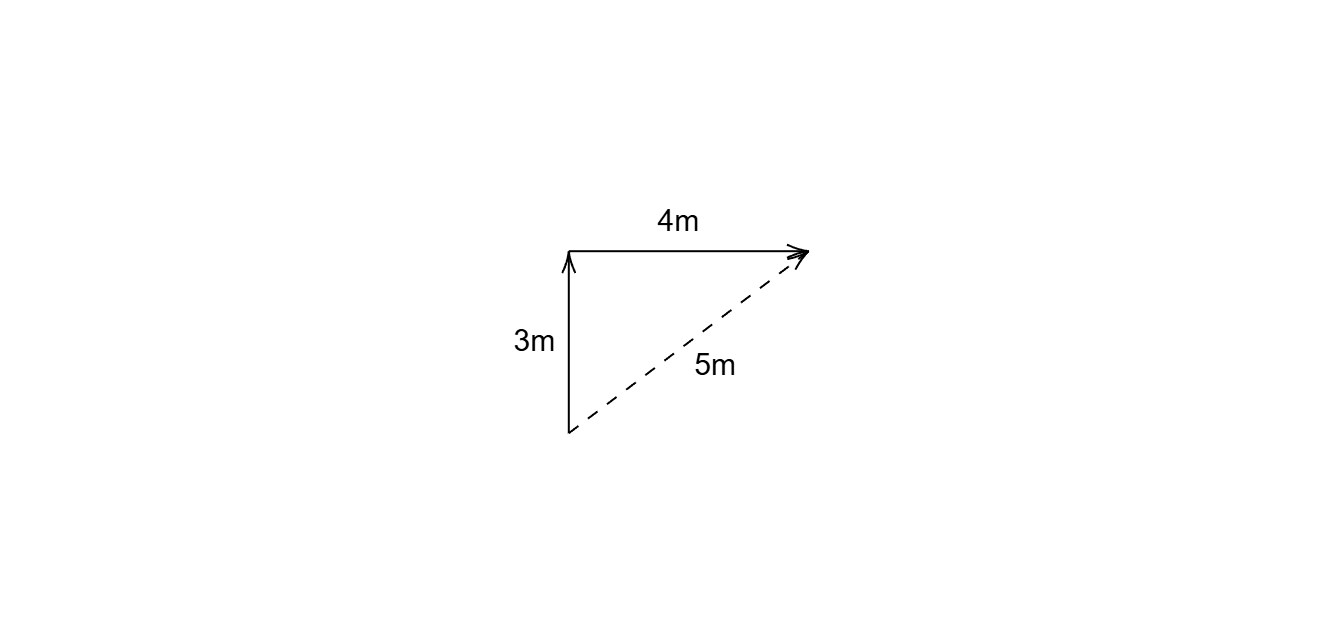
\includegraphics[width=0.5\textwidth]{Tuan2/Figures/gioithieuvector.png}
\end{figure}
Chúng ta sẽ làm việc với những bài toán như vậy khá nhiều, vì vậy sẽ là cần thiết để định nghĩa một đối tượng toán học có thể mô tả cả độ lớn và hướng. Đối tượng này được gọi là \textbf{vector}.
\begin{definition} Vector \(AB\) (hình vẽ), kí hiệu là \(\overrightarrow{AB}\), là một mũi tên được đặc trưng bởi độ dài \(a\) của nó (do đó còn được kí hiệu là \(\overrightarrow{a}\)) và hướng mà nó chỉ.
\end{definition}
\begin{figure}
\centering
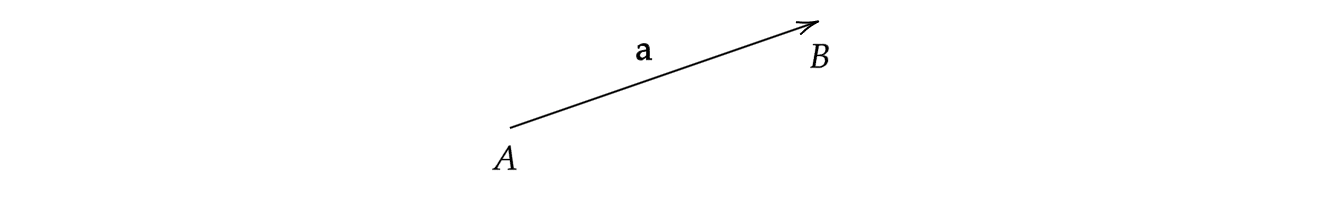
\includegraphics[width=0.5\textwidth]{Tuan2/Figures/vectorAB.png}
\end{figure}


